96. \begin{figure}[ht!]
\center{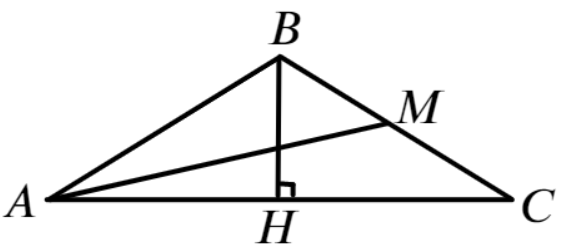
\includegraphics[scale=0.35]{g9-96.png}}
\end{figure}\\
Найдём $\angle C=(180^\circ-120^\circ):2=30^\circ.$ Тогда  $HC=\cfrac{1}{2}AC=\sqrt{2},\ AB=BC=\cfrac{HC}{\cos(30^\circ)}=\cfrac{\sqrt{2}}{\cfrac{\sqrt{3}}{2}}=\cfrac{2\sqrt{6}}{3}.$ По теореме косинусов для треугольника $ABM$ получим $BM=\sqrt{\cfrac{24}{9}+\cfrac{6}{9}-2\cdot\cfrac{2\sqrt{6}}{3}\cdot\cfrac{\sqrt{6}}{3}\cdot\left(-\cfrac{1}{2}
ight)}=\cfrac{\sqrt{42}}{3}.$
ewpage
oindent
